
%----------------------------------------------------------------------------------------
% Bachelorthesis. Andrew, Louis.
% Template by: Prof. C. Schmidt 	 
%----------------------------------------------------------------------------------------
\documentclass[oneside,bibliography=totocnumbered,BCOR=5mm]{scrbook}% Voreinstellungen entfernt.

\usepackage[latin1]{inputenc}
\usepackage{amsmath, amsthm, amssymb}
\usepackage[english]{babel} % Language hyphenation and typographical rules
\usepackage{marvosym}
\usepackage{graphics}
\usepackage{csquotes}
\newtheorem{satz}{Satz}[chapter]
\theoremstyle{definition} 
\newtheorem{definition}[satz]{Definition} 
\theoremstyle{definition} 
\newtheorem{lemma}[satz]{Lemma} 
\theoremstyle{definition} 
\newtheorem{bemerkung}[satz]{Bemerkung}
\theoremstyle{definition} 
\newtheorem{korollar}[satz]{Korollar} 
\theoremstyle{definition}
\newtheorem{beispiel}[satz]{Beispiel} 
\theoremstyle{definition} 
\newtheorem{algorithmus}{Algorithmus} 
\newenvironment{beweis}{\begin{proof}[Beweis]}{\end{proof}}
\usepackage[hyphens]{url}
\usepackage{hyperref}

\usepackage[backend=bibtex, style=numeric]{biblatex}
\addbibresource{template.bib}

\usepackage{blindtext} % Package to generate dummy text throughout this template 

\usepackage[sc]{mathpazo} % Use the Palatino font
\usepackage[T1]{fontenc} % Use 8-bit encoding that has 256 glyphs
\linespread{1.05} % Line spacing - Palatino needs more space between lines
\usepackage{microtype} % Slightly tweak font spacing for aesthetics

\usepackage[hmarginratio=1:1,top=32mm,columnsep=20pt]{geometry} % Document margins
\usepackage[hang, small,labelfont=bf,up,textfont=it,up]{caption} % Custom captions under/above floats in tables or figures
\usepackage{booktabs} % Horizontal rules in tables
\usepackage{lettrine} % The lettrine is the first enlarged letter at the beginning of the text
\usepackage{enumitem} % Customized lists
\setlist[itemize]{noitemsep} % Make itemize lists more compact

\usepackage{titling} 

\usepackage{listings}
\usepackage{color}

\usepackage{xcolor}

\usepackage{graphicx} % Readjust height and width of images
\usepackage{float} % Makes the figure float?!
\usepackage{hyperref}

\definecolor{lightgray}{rgb}{.9,.9,.9}
\definecolor{darkgray}{rgb}{.4,.4,.4}
\definecolor{purple}{rgb}{0.65, 0.12, 0.82}

\definecolor{eclipseStrings}{RGB}{42,0.0,255}
\definecolor{eclipseKeywords}{RGB}{127,0,85}
\colorlet{numb}{magenta!60!black}

\lstdefinelanguage{json}{
    basicstyle=\normalfont\ttfamily,
    commentstyle=\color{eclipseStrings}, % style of comment
    stringstyle=\color{eclipseKeywords}, % style of strings
    numbers=left,
    numberstyle=\scriptsize,
    stepnumber=1,
    numbersep=8pt,
    showstringspaces=false,
    breaklines=true,
    frame=lines,
    backgroundcolor=\color{lightgray}, %only if you like
    string=[s]{"}{"},
    comment=[l]{:\ "},
    morecomment=[l]{:"},
    literate=
        *{0}{{{\color{numb}0}}}{1}
         {1}{{{\color{numb}1}}}{1}
         {2}{{{\color{numb}2}}}{1}
         {3}{{{\color{numb}3}}}{1}
         {4}{{{\color{numb}4}}}{1}
         {5}{{{\color{numb}5}}}{1}
         {6}{{{\color{numb}6}}}{1}
         {7}{{{\color{numb}7}}}{1}
         {8}{{{\color{numb}8}}}{1}
         {9}{{{\color{numb}9}}}{1}
}

\lstdefinelanguage{JavaScript}{
  keywords={typeof, new, true, false, catch, function, return, null, catch, switch, const, if, in, while, do, else, case, break},
  keywordstyle=\color{blue}\bfseries,
  ndkeywords={class, export, boolean, throw, implements, import, this},
  ndkeywordstyle=\color{darkgray}\bfseries,
  identifierstyle=\color{black},
  sensitive=false,
  comment=[l]{//},
  morecomment=[s]{/*}{*/},
  commentstyle=\color{purple}\ttfamily,
  stringstyle=\color{red}\ttfamily,
  morestring=[b]',
  morestring=[b]"
}

\lstset{
   language=JavaScript,
   backgroundcolor=\color{lightgray},
   extendedchars=true,
   basicstyle=\normalfont\ttfamily,
   showstringspaces=false,
   showspaces=false,
   numbers=left,
   numberstyle=\footnotesize,
   numbersep=9pt,
   tabsize=2,
   breaklines=true,
   showtabs=false,
   captionpos=b,
   xleftmargin=0.5cm,
   aboveskip=0.5cm
}

\begin{document}

% Titelseite
% \pagestyle{empty}       % keine Seitennummer
\begin{titlepage}
\begin{center}

\includegraphics{images/HTW_Berlin_Logo_farbig.jpg}
\linebreak[4]
\linebreak[4]
\linebreak[4]
\linebreak[4]
\textit{\large Design \& Implementation of a Fraud Detection System for Autonomous Teams (Total pages should be: 50 [without Attachments])}
\linebreak[4]
\linebreak[4]
\linebreak[4]
Abschlussarbeit 
\linebreak[4]
\linebreak[4]
zur Erlangung des akademischen Grades: 
\linebreak[4]
\linebreak[4]
\textbf{Bachelor of Science (B.Sc.)} 
\linebreak[4]
\linebreak[4]
an der
\linebreak[4]
\linebreak[4]
Hochschule f\"ur Technik und Wirtschaft (HTW) Berlin
\linebreak[4]
Fachbereich 4: Informatik, Kommunikation und Wirtschaft
\linebreak[4]
Studiengang \textit{Angewandte Informatik}
\linebreak[4]
\linebreak[4]
\linebreak[4]
1. Gutachterin: Prof. Dr. Christin Schmidt\linebreak[4]
2. Gutachter: MSc. Tobias Dumke\linebreak[4]
\linebreak[4]
\linebreak[4]
\linebreak[4]
\linebreak[4]
Eingereicht von Louis Andrew [s0570624]
\linebreak[4]
\linebreak[4]
\linebreak[4]
\linebreak[4]
Datum
\linebreak[4]
\input{others/version}

\end{center}
\end{titlepage}

\newpage
\thispagestyle{empty}       % keine Seitennummer

\section*{Abstract}
[Summary of the thesis]



\clearpage
\pagenumbering{roman}% Seitennummerierung "roemisch"

\tableofcontents  

 \listoffigures

 \listoftables

 \lstlistoflistings

\newpage

\pagenumbering{arabic}  
 
\chapter{Introduction}

Fraud is an activity where someone intentionally deceives another person / system for any unlawful gain. The need to prevent as many fraud activities as possible should be one of the main priorities for businesses, as the number of fraud cases increase every year. In year 2021, the US Federal Trade Commission (FTC) received 2.8 million fraud reports, 70\% more in comparison to the fraud reports in 2020 \autocite{ftc}. Many businesses might already have some experience in handling such fraud cases, but an automated system that could detect and possibly prevent fraud activity with minimal supervision would be beneficial to reduce future risks while providing the possibility and capacity to scale their product.

Fraud detection system (FDS) is a system or program that uses a set of processes or techniques to detect fraudulent activities based on the input data in an automated way. FDS could possibly prevent further fraud activities by running a certain action (e.g. Blocking a fraudulent customer). 

As a business scale, it is often a good idea to split the responsibility of a certain domain to its own team, consisting of several people that focus solely on the given area. Large businesses are often built on top of multiple teams, working together as a whole, but usually handle their own responsibility, have their own goals and use a different technology stack and practices. Given the architecture principles and the autonomy of the teams, how could fraud detection and prevention centrally be managed?

\section{Background and Motivation}
The background and motivation of the thesis is to get my bachelor degree.
\section{Goal}
Goal of the thesis is to build a cool software
\section{Scope}

  The main purpose of this research project is to explore any possibility to facilitate a collaboration for several autonomous teams in a single fraud detection process while also providing crucial functionalities such as a notification system. 

  This project won't necessarily undertake aspects such as GDPR compliance and authentication of the system. Therefore, the system is not ready for production and further improvements on these aspects is required. The result of this research project is an explorative work, and may be used as a base for future projects in similar domain.  
\chapter{Grundlagen}
[Beschreibung des Kontextes der Arbeit mit allen durch die Problemstellung tangierten Bereichen, Methoden, Theorien, Erkenntnissen, Technologien, ... ] 


\section{Kontext}


\subsection{Domain} 



\subsection{Technologien}


\subsection{Methoden und Konzepte}


\section{...}


\subsection{...}


\subsection{...}
\chapter{Requirement Analysis (!)}
[Beschreibung der Erhebung, Granularisierung und Priorisierung der zu Grunde liegenden Anforderungen]

\section{Goal}

  The goal of the research project is to build a fraud detection system that provides a possibility for different teams to contribute on the fraud detection process independently, based on their views and knowledge on the characteristics of a potentially fraudulent customer. In such a way, the system can help in transforming the fraud detection process to be a collaborative process and each team make a contribution by making it more reliable as their knowledge increases. The system should enable collaboration across autonomous teams in a fraud detection process and simplify it by encapsulating the internal logic while presenting the result in an understandable format. The system is responsible primarily in determining whether a customer is likely fraudulent based on the information contributed by the different teams and notifying the concerned parties on certain cases when needed.
\section{Application Environment}

\section{State of the Art}

  Fraud detection and prevention intrinsically is a big topic. There are many scientific papers published regarding fraud detection / prevention, suggesting approaches with different methods and algorithms to create a system that could predict a fraud case as accurately as possible. 

  There are also quite a lot of service providers that offer a tailor-built fraud detection system, usually works using machine learning to analyze the data provided to the system. 
  
  However, this research project intends neither to come up with a new technique to better predict a fraud case nor to compete with the existing service providers, but rather to explore a possibility of how the domain knowledge from multiple independent teams can be combined to produce a reliable fraud detection system, enabling collaboration across different domains.


\section{Requirements}

  This chapter lists the requirements of the system by extracting the use cases from the goal of the research project and its priorities. 

  \subsection{Use Cases}
    \label{use_cases}

    A use case diagram is created to better visualize the flow and possible use cases of the system on a high level based on the goal of the research project.

    \begin{figure}[!ht]
     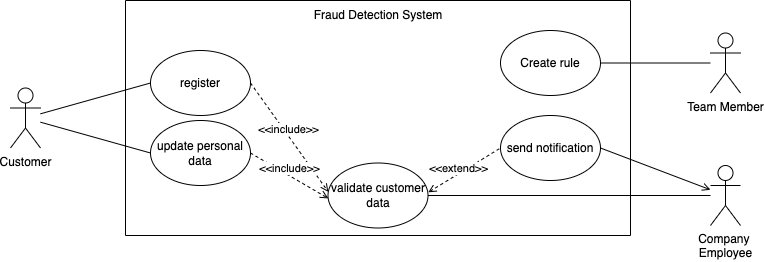
\includegraphics[width=\textwidth]{diagrams/use-case-diagram.png}
     \caption{Use case diagram of the fraud detection system}
     \label{fig:use_cases}
    \end{figure}

    The use case diagram gives a visual representation of the main functionality of the system as well as the actor involved in the process. The customer data validation will be run whenever a customer registers or updates his/her personal data. By running a validation whenever an operation on personal data is executed, the system would ideally validate and identify fraudulent customer as soon as possible. 
    
    Whenever a fraudulent customer is identified, a notification will be sent to concerned parties, so that necessary actions (for example, blocking the customer) can be taken as soon as possible. 

    The diagram also visualizes a use case of a validation rule creation by a team member, as a form of contribution based on his/her knowledge of a fraudulent customer with the intention to improve the reliability of the validation process.
    
  \newpage
  \subsection{User Stories}
    \label{user_stories}

    Based on the use cases visualized on \autoref{fig:use_cases}, the following user stories can be defined:

    \begin{itemize}
      \item \textbf{Verifying Customer Early}
        \begin{itemize}[label={},leftmargin=*]
          \item As a stakeholder, I want to verify customers, so that the company can have more confidence that the existing user base is trustworthy 
        \end{itemize}

      \item \textbf{Notification on Suspicious Cases}
        \begin{itemize}[label={},leftmargin=*]
          \item As an employee, I want to be notified when a user seems suspicious, so that I can do necessary actions accordingly
        \end{itemize}

      \item \textbf{Validation Rules Management}
        \begin{itemize}[label={},leftmargin=*]
          \item As an employee, I want to manage my own rule to validate users, so that I can use my expertise to find suspicious customers as efficiently as possible without the communication overhead with other teams
        \end{itemize}
    \end{itemize}

    The user stories listed above are the main requirements of the system. The functionalities of the system will be defined and implemented based on these user stories.
    
  \subsection{Software Quality Standard}
    \label{criteria}

    The system and software quality models defined in ISO 25010 \autocite{iso-2011} are used to establish a base on how to evaluate the quality of the system made for this research project. The table below contains a list of criteria taken from the software quality characteristics and its sub-characteristics described in ISO 20510, the meaning of each sub-characteristic and its importance to the research project. The criteria will be revisited during evaluation to assess the quality of the software made during the research project. 

     \begin{tabularx}{\linewidth}{p{0.3\textwidth} p{0.5\textwidth} p{0.2\textwidth}}
       \caption{Systems and software quality standard based on ISO 25010 and its importance} \\
        \toprule
        & Overview & Importance \\
        \midrule

        \multicolumn{3}{@{}l}{\textbf{Functional stability}}\\
        Completeness & System covers all the specified tasks listed on the requirement analysis & Very important \\
        Correctness & System provides correct results of the tasks listed on the requirement analysis & Very important \\
        Appropriateness & System accomplishes to fulfill the tasks listed on the requirement analysis in a well manner & Important \\

        \multicolumn{3}{@{}l}{\textbf{Reliability}}\\
        Maturity & System is stable during every day use & Important \\
        Availability & System is operational and accessible (ideally via a web browser and no installation is needed) & Very important \\
        Fault tolerance & System still operates well enough, despite software fault & Important \\
        Recoverability & System can recover data in the event of an interruption or failure & Very important \\

        \multicolumn{3}{@{}l}{\textbf{Performance efficiency}}\\
        Time behavior & Response and processing time of the system is reasonable & Important \\
        Resource Utilization & The amount and types of resources used by the system is kept as minimum as possible & Not important \\
        Capacity & Maximum limits of a system parameter is within a reasonable range for everyday use & Not important \\

        \multicolumn{3}{@{}l}{\textbf{Usability}}\\
        Appropriateness Recognizability & It can be easily recognized, that the system is suitable for the current user need & Not important \\
        Learnability & It's easy to learn how to use the system & Not important \\
        Operability & The system is easy to operate & Very important \\
        User Error Protection & System can protect or prevent users against making errors &Somewhat important \\
        User Interface Aesthetics & User interface is aesthetically pleasing & Very important \\
        Accessibility & System can be used with the widest range of characteristics and capabilities & Not important \\

        \multicolumn{3}{@{}l}{\textbf{Security}}\\
        Confidentiality & System is able to ensure that data is only accessible to those who have authorized access &Somewhat important \\
        Integrity & System is able to prevent unauthorized access and modification to computer programs &Somewhat important \\
        Non-repudiation & Actions or events can be proven to have taken place & Somewhat important \\
        Accountability & Actions of an unauthorized user can be traced back & Not important \\
        Authenticity & How well the identity of a subject / resource can be proved & Not important \\

        \multicolumn{3}{@{}l}{\textbf{Compatibility}}\\
        Co-existence & Each component of the system can work efficiently without any bottleneck while sharing the same environment & Somewhat important \\
        Interoperability & Two or more systems, products, or components are able to exchange information and use it & Very important \\

        \multicolumn{3}{@{}l}{\textbf{Maintainability}}\\
        Modularity & Component of system can be changed with minimal impact on the other component & Important \\
        Reusability & Assets can be used in more than one component & Not important \\ 
        Analysability & Activities within the system can be easily analyzed (e.g.: in form of logging) & Somewhat important \\
        Modifiability & System can be modified without introducing defects or degrading existing product quality & Very important \\
        Testability & Test criteria for a system is effective and preferably can be run automatically & Very important \\

        \multicolumn{3}{@{}l}{\textbf{Portability}}\\
        Adaptability & System can be adapted for different or evolving HW, SW or other usage environment & Not important \\
        Installability & System can be un- and/or installed successfully & Important \\
        Replaceability & System as a product can replace another comparable product & Not important \\

        \bottomrule
      \end{tabularx}

      \newpage

    

Optionals:
\begin{itemize}
 \item \textit{Rahmenbedingung}
 \item Methods
\end{itemize}
\chapter{Konzeption \& Entwurf}
[Beschreibung des Entwurfs auf Basis der Methodologie / der geplanten Vorgehensweise zur Probleml\"osung im Kontext der Anforderungen (i.A. der Art der Arbeit)]
\section{Prozess}
\section{Systemarchitektur}
\section{Softwarearchitektur}
\section{Schnittstellen}
\section{Datenmanagement}
\section{...}
\chapter{Implementation}

As the design of the system is defined and the functionalities of each component of the system is clear, the implementation of the system can finally start. This chapter describes the detailed information on the implementation of the structure and functionalities listed in \autoref{chapter:concept}.


\section{Technologies and Architecture}

Before implementing a specific functionality of the system, each component of the system needs to be setup and configured, so that an iterative development process can be done correctly. The prerequisites that need to be met before setting up the projects are: 

\begin{itemize}
 \item Node.JS version 16 is installed
 \item NPM is installed
 \item Docker is installed
 \item Git is installed
\end{itemize}

For certain components of the system, a live environment is configured, so that the system is accessible via a URL, without having to set it up on a local machine. 


 \subsection{User Interface}
 As mentioned in \autoref{concept_ui}, the UI is a web application, built using Vue3 and TypeScript.

  \subsubsection{Setup}
   Nowadays, most front end projects use some kind of build tool to help build, test, and develop web applications\footnote{For detailed information on the role of a build tool in front end development, please take a look at \autocite{Odell2014}}. The build tool \emph{Vite}\footnote{\emph{Vite} is an open source front end build tool. GitHub repository: \url{https://github.com/vitejs/vite}} is used to build, test and develop the UI. A new Vite project is created by running the following command in a shell terminal:
  
  \begin{lstlisting}[caption={Creating a new Vite project (Shell)}]
 npm create vite@latest ui --template vue-ts
  \end{lstlisting}

  A version control to track and manage the progress done in this particular project is also used. The version control used in this project is git and a code hosting platform for version control is also used for the project (GitHub).

  \subsubsection{Component Library}
  A component library is used in this project to speed up the development. The component library used in this project is \emph{NaiveUI}\footnote{\emph{NaiveUI} is a Vue3 component library. GitHub repository: \url{https://github.com/TuSimple/naive-ui}}. NaiveUI is chosen because it contains several components that are suitable for the project (for example: \textsc{Timeline}, \textsc{Menu}) and it also supports TypeScript out of the box.

  \subsubsection{Code Style}
  To enforce a consistent code style and comply to the best practices of a TypeScript project, a code formatter (\emph{Prettier}) and linter (\emph{ESLint}) are used in this project. 

  \subsubsection{Docker}
  \textbf{TODO. Implementation not done}

  \subsubsection{CI/CD}
  A CI/CD process is configured within the project, to run certain actions on specific events that happen in the codebase. The tool used to enable this functionality is \emph{GitHub actions}\footnote{\emph{GitHub actions} is a CI/CD platform, created by GitHub and can be used in all repositories hosted on GitHub. Homepage: \url{https://github.com/features/actions}}. The configured CI/CD actions in this project are:

   \begin{itemize}
    \item Run test and build, when there's a new pull request (PR)\footnote{\emph{Pull request (PR)} is a request from a developer to merge certain changes on a dedicated branch to the main branch of a repository} to \emph{main} branch
    \item Run release and bump version of the app, when there's a new commit to \emph{main} branch
   \end{itemize}
  
  \subsubsection{Deployment}
  A live environment is available for the UI. The live environment is made possible by using \emph{Netlify}\footnote{\emph{Netlify} is a hosting platform with a git-based workflow. Homepage: \url{https://www.netlify.com/}}. Every change made to the \emph{main} branch will be built and deployed on the Netlify platform automatically. 

 \subsection{FDS}
 As described in \autoref{concept_fds}, the FDS is a server side application, built with Node.JS and TypeScript. To build a REST API with ease, the Express.JS framework will also be used in this project. 

  \subsubsection{Setup}
  To set up a new Node.JS project, run the following command in a shell terminal:

   \begin{lstlisting}[caption={Creating a new Node.JS program (Shell)}]
 mkdir fds
 cd ./fds
 npm init -y
   \end{lstlisting}
   
  To use the TypeScript language rather than plain JavaScript, the TypeScript compiler needs to be installed and used in this project. The TypeScript compiler can also be configured to be more suitable to the personal preferences of the developer as well as the requirements of third party libraries used by the project. To install TypeScript as a development dependency\footnote{In a Node.JS project, development dependency is a third party library used only for development purposes} and to initiate the configuration file of the TypeScript compiler, run the following commands in a shell terminal:
  
   \begin{lstlisting}[caption={Installing and configuring TypeScript compiler (Shell)}]
 npm i -D typescript
 tsc --init
   \end{lstlisting}
  
  To install Express.JS in the current project, run the following command in a shell terminal:
  
   \begin{lstlisting}[caption={Installing Express.JS (Shell)}]
 npm i express
   \end{lstlisting}
  
  \subsubsection{Tsoa and Swagger}
  Even though Express.JS provides a declarative and easy way to build a server side application, it's built with JavaScript in mind. Therefore, even though TypeScript can be used with Express.JS, it doesn't use all the potential functionalities that TypeScript provides. \emph{Tsoa}\footnote{\emph{Tsoa} GitHub repository: \url{https://github.com/lukeautry/tsoa}} is a framework with integrated openAPI compiler to build server side applications that can leverage TypeScript to its potential. \emph{Tsoa} helps an express application to have the following functionalities out of the box:

   \begin{itemize}
    \item Generate Swagger\footnote{\emph{Swagger} is a tool to document server side APIs. Homepage: \url{https://swagger.io/}} specification based on HTTP controller code
    \item Generate Swagger schema based on TypeScript interfaces
    \item Generate Swagger schema descriptions based on \emph{jsDoc}\footnote{\emph{jsDoc} is a tool to generate API documentation, similar to \emph{JavaDoc}. Homepage: \url{https://jsdoc.app/}} comments on the source code
   \end{itemize}
  
  Other than that, \emph{tsoa} provides an alternative syntax to build an Express.JS application in a more object-oriented way. \emph{Tsoa} works by compiling the code, with the help of the TypeScript compiler into a regular Express.JS application, built with JavaScript. 

  \subsubsection{Code Style}
  Identical to the UI project, a code formatter (\emph{Prettier}) and linter (\emph{ESLint}) are also used in this project. The configuration for the code formatter and linter is slightly different in comparison to the UI project, as certain code style rules doesn't apply to a server side application\footnote{In the UI project, there are certain code style rules regarding HTML elements}.

  \subsubsection{Docker}
  The application will be built and run as a Docker container. To be able to run an application as a Docker container, a \emph{Dockerfile} is needed as a list commands needed to be run to assemble the particular image. The commands used to assemble a Docker container for the FDS are:

   \begin{lstlisting}[caption={Dockerfile for FDS (Docker)}, language=docker]
 FROM node:16-alpine

 ARG ARG_1 # Arguments passed by --build-args flag
 ENV ARG_1=$ARG_1 # Environment variable of the image

 WORKDIR /app
 COPY ["package.json", "package-lock.json*", "./"]

 RUN npm ci # Install packages
 COPY . .
 # Additional steps to setup the application

 RUN npm run build
 ENV NODE_ENV=production

 CMD [ "node", "./dist/src/main.js" ]
   \end{lstlisting}
  
  \subsubsection{CI/CD}
  A CI/CD process is also configured for this project using GitHub actions. The actions configured in this project are:

   \begin{itemize}
    \item Run test and build, when there's a new PR to the \emph{main} branch
    \item Run release, bump version of the application and deploy it to the live environment, when there's a new commit to \emph{main} branch
   \end{itemize}
   
  \subsubsection{Deployment}
  A live environment is available for the FDS application. The FDS is deployed and run as a Docker container in \emph{Heroku}\footnote{\emph{Heroku} is a platform as a service (PaaS) that provides a platform for developer to build and run application in the cloud. Homepage: \url{https://heroku.com}}. The deployment process will be executed via the CI/CD action on every commit to the \emph{main} branch. 

 \subsection{RabbitMQ}
 A RabbitMQ instance is required as one of the integral parts of the system. Fortunately, RabbitMQ provided an official Docker image for it and running a RabbitMQ instance as a Docker container is as simple as running the following command in a shell terminal:

 \begin{lstlisting}[caption={Running a RabbitMQ instance with Docker (Shell)}]
 docker run -it --rm --name rabbitmq -p 5672:5672 -p 15672:15672 rabbitmq:3.10-management 
 \end{lstlisting}

 The command listed above will locally run the RabbitMQ instance on port \emph{5672} and the RabbitMQ management UI on port \emph{15672}. On the live environment, a service called \emph{CloudAMQP}\footnote{\emph{CloudAMQP} is a service provider (RabbitMQ as a Service) that offers RabbitMQ clusters setup and management} is used to help in setting up a RabbitMQ instance in the cloud, so that it can be accessed by other components via its public URI easily.

 \subsection{Redis}
 Redis is used in the system as a caching memory and a temporary data store. Redis also provided an official Docker image. To run a Redis instance as a Docker container, the following command should be run in a shell terminal:

 \begin{lstlisting}[caption={Running a Redis instance with Docker (Shell)}]
 docker run -d --name redis-stack-server -p 6379:6379 redis/redis-stack-server:latest
 \end{lstlisting}

 The command listed above will locally run the Redis instance in port \emph{6379}. Redis is not available on the live environment. On the live environment, no caching is available and an in memory data store (a basic JavaScript class) is used to replace Redis.

 \subsection{MongoDB}
 MongoDB is the database of choice for the system. MongoDB has an official Docker image and the following command should be run in a shell terminal to set up a MongoDB instance locally:

 \begin{lstlisting}[caption={Running a MongoDB instance with Docker (Shell)}]
 docker run --name mongodb -d -p 27017:27017 mongo 
 \end{lstlisting}

 By running the command listed above, a MongoDB instance will be run locally on port \emph{27017}. On the live environment, a service called \emph{MongoDB Atlas}\footnote{\emph{MongoDB Atlas} is a service that provides a cloud-hosted MongoDB instances. Homepage: \url{https://www.mongodb.com/atlas}} will be used to help host a MongoDB instance in the cloud, making it more accessible by other components of the system.

 \subsection{Docker Compose}
 \textbf{TODO. Implementation not done}


\section{Object Models}
  \label{impl_model}

In this chapter, the specific implementation of the object models described in \autoref{subsection:model} will be discussed. 

  \subsection{Validation Rule}
    \label{impl_model:rule}

    The subsection describes the implementation of the \verb;ValidationRule; object model as a TypeScript interface.

    \subsubsection{Retry Strategy}
      \label{impl_model:rule__retry}

      The \verb;retryStrategy; attribute of the validation rule model is very specific to the implementation of the FDS. The FDS is using a library called \emph{Got}\footnote{\emph{Got} is a Node.JS library to make HTTP requests. GitHub repository: \url{https://github.com/sindresorhus/got}.} to make HTTP requests to the external endpoints. Got provides the functionality to retry a failed HTTP request out of the box\footnote{For more information on Got's retry options, please refer to \url{https://github.com/sindresorhus/got/blob/main/documentation/7-retry.md}.}.

      The \verb;retryStrategy; attribute of a validation rule is a subset of the retry options provided by Got's retry API, and will be passed to the Got instance when the HTTP request is made for the corresponding rule evaluation. 

    \subsubsection{TypeScript interface}
      As the implementation of the model defined in \autoref{fig:uml_validation_rule}, a TypeScript interface is created to provide a clear structure of a validation rule.

      \begin{lstlisting}[style=es6, caption={TypeScript interface of a validation rule (TypeScript)}]
export interface ValidationRule {
  retryStrategy?: RetryStrategy | null
  requestUrlParameter?: GenericObject
  requestHeader?: GenericObject
  skip: boolean
  requestBody?: GenericObject
  condition: Condition | BooleanCondition
  method: "GET" | "PUT" | "POST" 
  failScore: number
  endpoint: string
  priority: number
  name: string
}

type GenericObject = { [key: string]: any } // Dictionary
type Condition = {
  path: string
  operator: OperatorType
  type: ConditionType
  value: any
  failMessage: string
}

type BooleanCondition = {
  all: Condition[]
} | {
  any: Condition[]
}

type RetryStrategy = {
  limit: number
  statusCodes: number[] 
}
      \end{lstlisting}

  \subsection{Validation Result}
  
    A TypeScript interface is created as the implementation of the validation result structure listed on \autoref{fig:uml_validation_result}. The FDS is not responsible in storing validation results in a database. Therefore, a Prisma schema won't be created for validation results. 

    \newpage
    \begin{lstlisting}[style=es6, caption={TypeScript interface of a validation result (TypeScript)}]
export interface Validation<T> {
  validationId: string
  fraudScore: number
  totalChecks: number
  runnedChecks: number
  skippedChecks: string[]
  additionalInfo: ValidationAdditionalInfo<T>
  events: ValidationEvent[]
}

export type ValidationEventStatus = "NOT_STARTED" | "FAILED" | "PASSED" | "RUNNING"
export type ValidationEvent = {
  name: string
  status: ValidationEventStatus
  dateStarted: string | null
  dateEnded: string | null
  messages?: string[]
}

export type ValidationAdditionalInfo<T> = {
  startDate: string
  endDate?: string
  customerInformation?: T
}
    \end{lstlisting}
\section{Controller}

  This chapter describes the implementation of the features elicited on the previous chapters in details, specifically within the FDS component. All the HTTP routes of the FDS will be prefixed with \verb;/api/v1;.

  \subsection{Customer Validation on a Registration Event}

    An HTTP endpoint will be implemented to provide the possibility to schedule a validation process as soon as a new customer is registered. The endpoint should accept the customer information on the request body and return validation ID and additional information of the validation process as a response. Listed below is the code snippet of the HTTP controller of the endpoint to schedule a validation process:

    \begin{lstlisting}[style=es6, caption={HTTP controller of an endpoint to schedule a validation process (TypeScript)}]
// fds/src/routes/validation/validationController.ts

// Picks the `validationId` and `additionalInfo` attributes from `Validation` 
type ValidationSchedule = Pick<Validation, "validationId" | "additionalInfo"> 
     
@Route("validate")
@Tags("Validation")
export class ValidationController extends Controller {
  @SuccessResponse(201, "Validation started")
  @Response<ValidationErrorJSON>(422, "Validation Failed")
  @Response<WentWrong>(400, "Bad Request")
  @Post()
  public async validateCustomer(
   @Body() requestBody: Customer
  ): Promise<ValidationSchedule | WentWrong> {
    const result = await ValidationService.scheduleRulesetValidation(requestBody)
    const { data, error } = result

    if (error) {
      this.setStatus(400)
      return {
        message: error.message,
        details: error.details || "",
      }
    }

    return data
  }
} 
    \end{lstlisting}
    
    The HTTP controller is intentionally kept as simple as possible. The logic behind the process to schedule a validation is done by the \verb;ValidationService; and \verb;ValidationEngine; (discussed in \autoref{sub:process}). The \verb;ValidationService; is responsible in this particular case to get the lists of existing validation rules and runtime secrets (discussed in \autoref{sub:secrets}), then creating a new instance of \verb;ValidationEngine; as well as scheduling a new validation process. 

    \begin{lstlisting}[style=es6, caption={ValidationService schedule validation implementation (TypeScript)}]
// fds/src/routes/validation/validationService.ts

export class ValidationService {
  static async scheduleRulesetValidation(
    customer: Customer
  ): Promise<ApiResponse<ValidationSchedule>> {
    const { data: ruleset, error } = await RulesService.listRules()
    const secrets = await SecretsService.listSecrets()
    if (error) {
      return {
        data: null,
        error,
      }
    }

    const { validationId, additionalInfo } = await new ValidationEngine<Customer>()
      .setRuleset(ruleset)
      .setSecrets(secrets)
      .scheduleRulesetValidation(customer)

    return {
      data: {
        validationId,
        additionalInfo,
      },
      error: null,
    }
  }
}
    \end{lstlisting}

  \subsection{Validation Process}
    \label{sub:process}

    \subsubsection{Validation Process Flow}
    
      A validation process is started by iterating through a list of validation rules, making an HTTP request to the external endpoint listed on each rule and evaluating its response in comparison to the conditions attached on the rule. If the HTTP response from the external matches the conditions of the rule, the rule evaluation will be considered as a passed evaluation, otherwise it is a failed evaluation. The result of each rule evaluation determines the value of the resulting fraud score. The resulting fraud score will be calculated as follows: 

      \begin{itemize}
        \item Initialize an empty list of fraud scores. The list will be filled later with float numbers ranging between 0 and 1
        \item Go through the list of validation rules and run evaluation
        \item If the evaluation passed, append \verb;0; to the list of fraud scores
        \item Otherwise, append the validation rule \verb;failScore; attribute's value to the list of fraud scores
        \item At the end of the iteration, the list size should equal to the amount of available\footnote{\emph{Not skipped.}} validation rules
        \item The resulting fraud score is the sum of the scores in the list, divided by the number of available validation rules
      \end{itemize}
      
      In summary, the flow of a validation process will be represented by the flow diagram below:

      \begin{figure}[!ht]
        \centering
        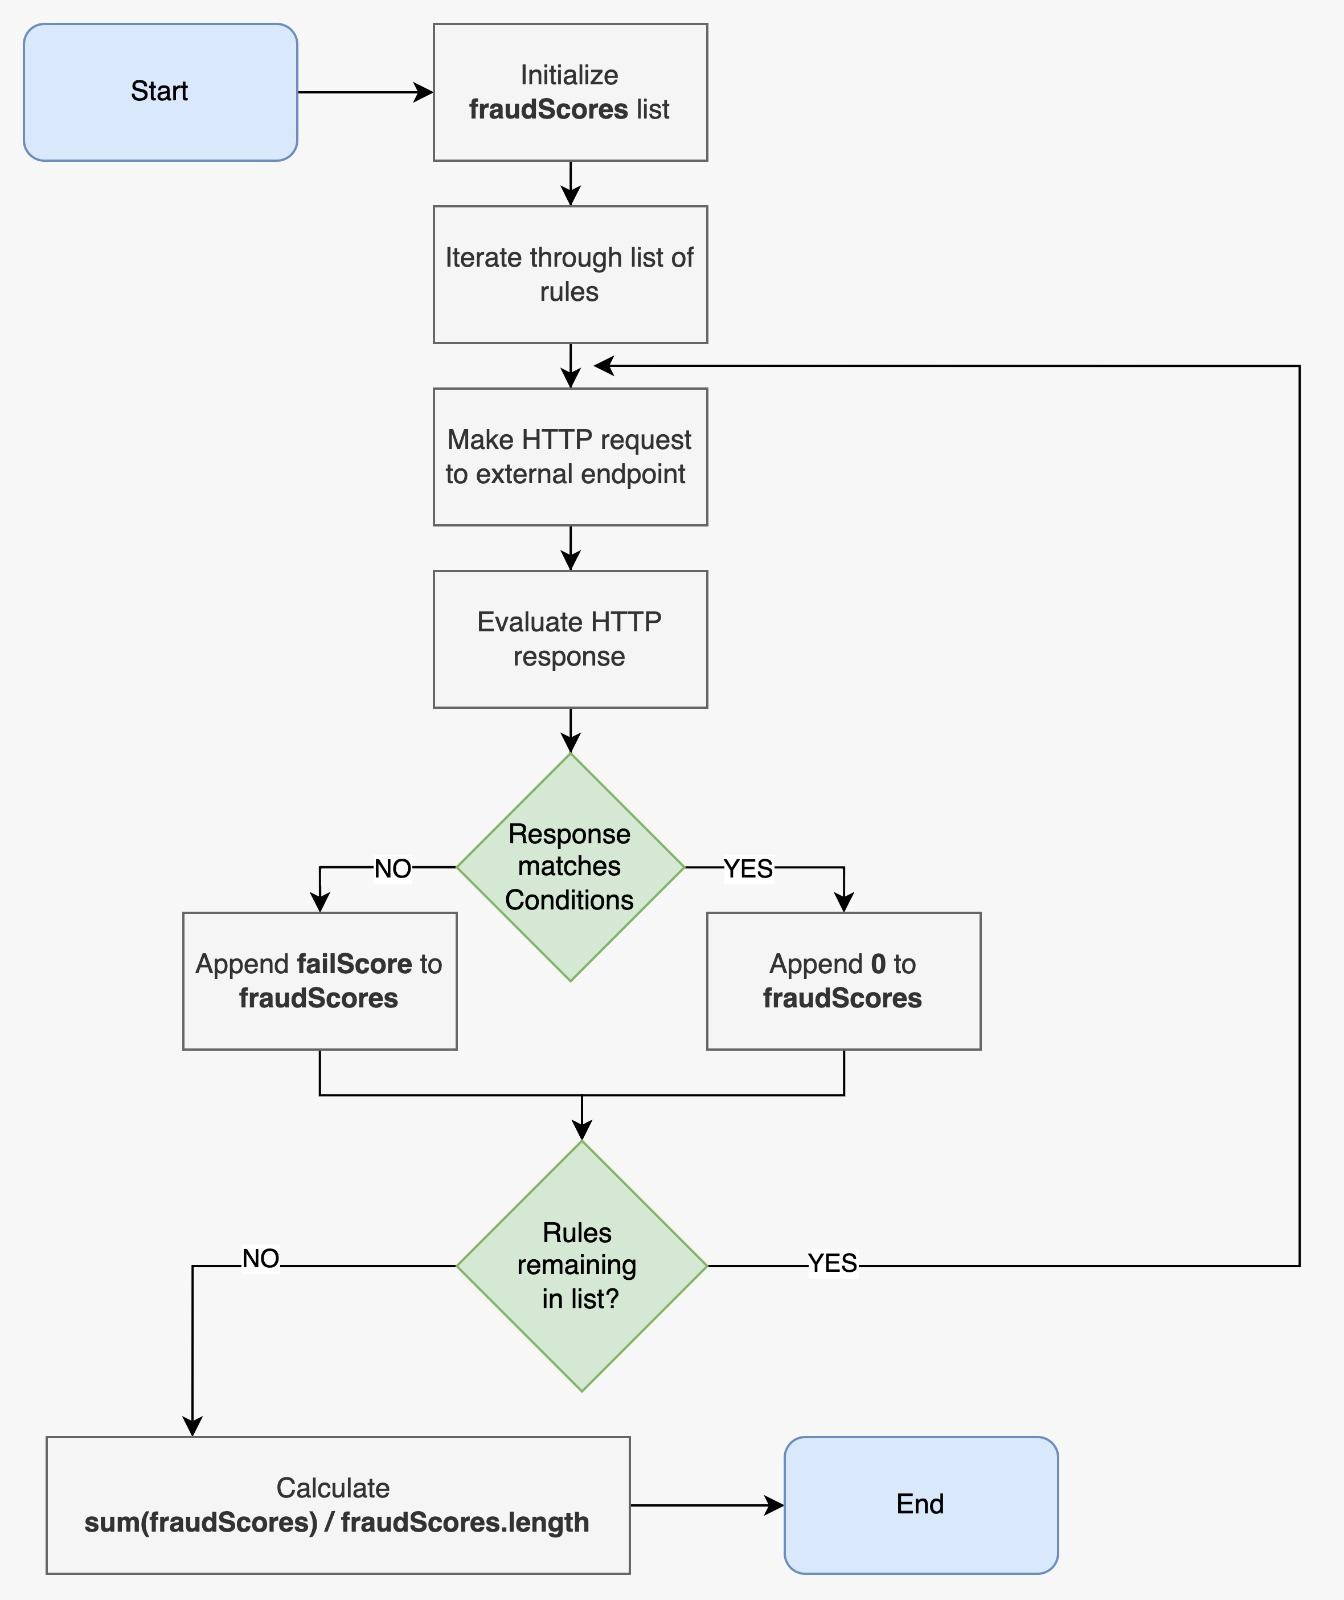
\includegraphics[width=0.8\textwidth]{diagrams/flow_validation_process.jpeg}
        \caption{Flow diagram of a validation process}
        \label{fig:flow_validation}
      \end{figure}
      
      The flow listed above will be executed by creating a \verb;ValidationEngine; instance and calling a public \verb;secheduleRulesetValidation; method. Before running a validation process, the list of validation rules as well as runtime secrets should be provided to the engine. The \verb;ValidationEngine; class uses method chaining\footnote{\emph{Method chaining} is a method to provide the possibility of invoking multiple method calls of an object without having to store an intermediary result in an additional variable.} as well as the \emph{Builder} design pattern discussed in \autocite[pp. 97-106]{gamma-1995} for its construction, to make the public API of a validation engine as simple as possible.

      \begin{lstlisting}[style=es6, caption={ValidationEngine class and the scheduleRulesetValidation method (TypeScript)}]
// fds/src/engine/valdiationEngine.ts
export class ValidationEngine<T> {
  private secrets: GenericObject = {}
  private ruleset: ValidationRule[] = []

  setSecrets(secrets: GenericObject) {
    this.secrets = secrets
    return this
  }

  setRuleset(ruleset: ValidationRule[]) {
    this.ruleset = [...ruleset.sort((a, b) => b.priority - a.priority)]
    return this
  }

  async scheduleRulesetValidation(data: T): Promise<Validation<T>> {
    if (this.ruleset.length === 0) {
      throw new Error("Ruleset is not set")
    }

    await this.constructValidationObject(data) // Construct a validation result
    this.validateRuleset(data)

    return this.validationResult
  }

  async validateRuleset(data: T): Promise<Validation<T>> {
    if (this.ruleset.length === 0) {
      throw new Error("Ruleset is not set")
    }

    if (!this.validation) {
      await this.constructValidationObject(data)
    }

    for await (const rule of this.ruleset.filter(({ skip }) => !skip)) {
      const evaluationResult = await this.evaluateRule(rule, data)
      await this.reviewEvaluationResult(evaluationResult, rule)
    }

    await this.afterValidation()

    return this.validationResult
  }
}
      \end{lstlisting}

    \subsubsection{Accessing Data by Evaluating JSONPath Expressions}
      
      To be able to access essential information stored in the current runtime scope a validation process, a JSONPath expression can be used in certain attributes of a validation rule. The provided runtime information of a validation process includes the customer information, runtime secrets and during a condition evaluation, the HTTP response from the external endpoint of the particular rule. 

      The ability to access certain information from the runtime scope is needed when an HTTP request is made and during the evaluation of a condition. To evaluate a JSONPath expression, the \verb;jsonpath; library is used. 

      \begin{lstlisting}[style=es6, caption={Accessing runtime information using JSONPath expression (TypeScript)}]
import jp from "jsonpath"

const accessDataFromPath = (runtimeData: any, expression: any) => {
  if (typeof expression !== "string") {
    return expression // A valid JSONPath expression is a string
  }
  
  try {
    const [dataFromPath] = jp.query(runtimeData, expression)
    if (!dataFromPath) {
      // Expression is valid, but the path doesn't point to a specific value
      return expression 
    }

    return dataFromPath
  } catch {
    return expression // The expression is either not a valid JSONPath expression
  }
}
      \end{lstlisting}

    \subsubsection{Making an HTTP Request to External Endpoints}

      A dedicated class (\verb;Agent;) is created to make an HTTP request to the external endpoint. The class will provide a layer of abstraction on top of the Got library that is being used to actually make the HTTP requests. 
      
      The class will also help in setting the request body, request header as well as to change the variables on the \verb;endpoint; attribute with its corresponding values. The class follows the \emph{Singleton} design pattern described in \autocite[pp. 127-134]{gamma-1995}, as there might only one instance needed for the whole application. The class is also implemented using the dependency injection in mind, for an easier access to the underlying library during the testing phase. The dependency injection is implemented by providing a \verb;context; object to the \verb;Agent; class beforehand. During runtime, the \verb;context; object contains a Got instance, used to make HTTP requests. In testing environment, the \verb;context; object contains a mocked Got instance.

      \begin{lstlisting}[style=es6, caption={Usage of the singleton pattern and dependency injection in Agent class (TypeScript)}]
export class Agent {
  private static context: Context // Dependency injection

  private static get client() {
    return Agent.context.client // `client` object is a Got instance
  }

  static setClient(context: Context) {
    this.context = context
  }
}
      \end{lstlisting}

    \subsubsection{Operators}

      \verb;Operators; are special classes that define the operation of a certain condition during a validation process. Each \verb;Operator; is grouped by its type and has two main properties \verb;identifier;, and \verb;operateFunction;
      
      The \verb;identifier; property of an operator refers to the operator's name, unique on its group of type. The \verb;identifier; attribute of an operator will be passed into the \verb;operator; attribute of a condition to describe the specific operator to be used in evaluating the particular condition. The \verb;operateFunction; attribute of an operator is a function that accepts two arguments, and returns a boolean value that indicates whether the operation is successful. An additional validation process is also implemented using the \verb;validateFunction; property to make sure that the value being passed into the \verb;operate; function of an operator is valid. The \verb;identifier; and \verb;operateFunction; attributes of an operator are passed into the object constructor during its initialization, while the \verb;validateFunction; attribute of an operator is defined by each subclass of the operator, grouped by its type.  
      
      \begin{lstlisting}[style=es6, caption={NumberOperator example (TypeScript)}]
export class NumberOperator extends Operator<number, NumberOperatorIds> {
  const validateFunction = (value) =>
    typeof value === "number" &&
    !isNaN(parseFloat(`${value}`))
}

export const numberOperators: Record<NumberOperatorIds, NumberOperator> = {
  eq: new NumberOperator("eq", (a, b) => b === a),
  gt: new NumberOperator("gt", (a, b) => b > a),
  gte: new NumberOperator("gte", (a, b) => b >= a),
  lt: new NumberOperator("lt", (a, b) => b < a),
  lte: new NumberOperator("lte", (a, b) => b <= a),
} 
      \end{lstlisting}

      The \emph{Flyweight} design pattern mentioned in \autocite[pp. 195-206]{gamma-1995} is used here, by instantiating all the available operators beforehand, and using the instantiated object during a condition evaluation. For an even easier access to the operators, a \emph{flyweight factory} is also created. The \verb;OperatorFactory; will return the appropriate operator to be used based on the type and identifier passed. If the combination of type and identifier of an operator doesn't point into a specific operator, a \verb;NullishOperator; will be returned, which always return \verb;false; as its operation result. 

    \subsubsection{Evaluating a Rule} 
      
      To evaluate a certain validation rule, the \verb;Evaluator; class is created. The \verb;Evaluator; class is responsible in running an evaluation regarding a certain condition. An evaluator works together with the \verb;Operator; class in evaluating the conditions given. The specific operator to evaluate a condition is accessed via the \verb;OperatorFactory;. The \verb;Evaluator; class encapsulates the internal logic of evaluating a condition and running the operations defined by the particular condition. The \verb;Evaluator; class is also responsible in accessing the required data described by a JSONPath expression from the runtime information of a validation process. 

      \begin{lstlisting}[style=es6, caption={The usage of OperatorFactory class in the Evaluator class (TypeScript)}]
// Evaluate JSONPath expressions.
const dataFromPath = this.accessDataFromPath(runtimeData, validationRule.path)
const valueFromPath = this.accessDataFromPath(runtimeData, validationRule.value)
        
const operator = OperatorFactory.getOperator(
  validationRule.type,
  validationRule.operator,
)
const isEvaluationPassed = operator.operate(valueFromPath, dataFromPath)
      \end{lstlisting}
      
      As mentioned before, a condition can either be a single condition, or multiple conditions, wrapped inside an \verb;any; or \verb;all; attribute. The evaluation of a single condition is different from the evaluation of multiple conditions. To facilitate the different logic of evaluating conditions, two subclasses of the \verb;Evaluator; class is created. \verb;ConditionEvaluator; is responsible in evaluating a single condition, while the \verb;BooleanConditionEvaluator; is in charge in evaluating multiple conditions and handling the logic behind evaluating the \verb;any; and \verb;all; modifier. To simplify the instantiation of the suitable \verb;Evaluator; subclass, the \verb;EvaluatorFactory; class is created, following the \emph{Factory Method} design pattern described in \autocite[pp. 107-116]{gamma-1995}. 

      \begin{lstlisting}[style=es6, caption={EvaluatorFactory usage in ValidationEngine class (TypeScript)}]
const response = await Agent.fireRequest(rule, {
  customer: customerData,
  secrets: this.secrets
})

const evaluator = EvaluatorFactory.getEvaluator(condition)
const evaluationResult = evaluator.evaluate({
  response: response.data,
  customer: customerData,
  secrets: this.secrets
})
      \end{lstlisting}

      As the evaluation result, an \verb;Evaluator; instance will return an object with the \verb;pass; attribute to determine whether the evaluation passed and an additional \verb;messages; attribute, which contains essential information regarding the evaluation (including the value of \verb;failMessage; attribute of a condition, if the evaluation fails). 

  \subsection{Notification on Suspicious Cases}
      
    In \autocite{amqp}, Subramoni et al. describes an exchange as a routing mediator that copies and send the message sent by a message publisher to zero or more message queues. The FDS acts as the message publisher of the system and publishes a message to a pre-defined exchange on every completion of a validation process. 
    An interface to access and publish a message to the exchange is implemented using the \emph{Singleton} \autocite[pp. 127-134]{gamma-1995} design pattern, to only have a single connection to the RabbitMQ, since an AMQP connection are designed to be long-lived and opening a new connection to a RabbitMQ instance is an expensive operation. The type of exchange used in the system is the \emph{fanout} exchange. When a message is published to a fanout exchange, the message will be routed to all the queues bound to the exchange, which is ideal for the use case of the current notification system. 

    \begin{lstlisting}[style=es6, caption={Openning a connection to RabbitMQ instance (TypeScript)}]
import { Channel, connect } from "amqplib"
export class Notification {
  private static channel: Channel | null = null

  async init(url: string) {
    try {
      const connection = await connect(url)
      const channel = await connection.createChannel() // Create a new channel
      // Assert whether the exchange exists, create new if it doesn't exist
      await channel.assertExchange("FDS", "fanout", {
        durable: true 
      }) 

      Notification.channel = channel
    } catch (err) {
      console.error(err)
    }
  }
}
    \end{lstlisting}
    
    The \verb;Notification; class also provides the \verb;publish; static method, which can be used to publish a new message to the exchange if the connection is opened successfully. The \verb;ValidationEngine; class calls the \verb;publish; method every time a validation process is completed, publishing the validation result of the particular validation process to the exchange.

    \begin{lstlisting}[style=es6, caption={Publishing a validation result to the RabbitMQ exchange (TypeScript)}]
Notification.publish(JSON.stringify(this.validationResult))
    \end{lstlisting}
    
    There can be many consumers consuming the messages published to the exchange, and run certain actions regarding the internal logic of the system itself. The message consumer can, for example email the concerned parties if the fraud score exceeds a certain threshold or even automatically block a customer if a specific rule evaluation failed. To consume a message published to the exchange, a connection to the RabbitMQ instance needs to be opened, and a dedicated message queue (ideally created only for internal usage of the consumer itself) is needed. 

    \begin{lstlisting}[style=es6, caption={Consuming a message published to the RabbitMQ exchange (TypeScript)}]
import { connect } from "amqplib"
export const start = async (url: string) => {
  try {
    const connection = await connect(url)
    const channel = await connection.createChannel()
    await channel.assertExchange("FDS", "fanout", { durable: true })
    // Create an exclusive queue (created only for internal usage)
    const { queue } = await channel.assertQueue("", { exclusive: true })

    // Bind the exclusive queue to the exchange
    channel.bindQueue(queue, "FDS", "") 

    await channel.consume(queue, async (message: string) => {
      // Do actions
    }, {
      noAck: true
    })
  } catch (err) {
    console.error(err)
  }
}
    \end{lstlisting}

  \subsection{Validation Rules Management}
  
    The management of validation rules are done via the ORM (Prisma). To be able to use the ORM, a connection to the database needs to be created beforehand. The \emph{Singleton} \autocite[pp. 127-134]{gamma-1995} design pattern is also used here to make sure, that only a single connection to the database is created. \emph{Dependency injection} is also used here to be able to provide a mocked Prisma instance during testing. 

    \begin{lstlisting}[style=es6, caption={ (TypeScript)}]
export class Database {
  private static context: Context

  private static get prisma(): PrismaClient {
    return this.context.prisma
  }

  constructor(context: Context) {
    Database.context = context
  }

  async init() {
    await Database.prisma.$connect()
  }
}
    \end{lstlisting}

    Caching can also be enabled in the \verb;Database; class, by providing a \verb;DataStore; instance to the static \verb;setCache; method. By enabling caching, the values retrieved and updated can be cached to provide a faster response time. 

  \subsection{Validation Real Time Progress}

  \subsection{Runtime Secrets}
    \label{sub:secrets} 

  \subsection{Error Handling}


\section{View}

  This chapter discusses the implementation of the features on the user interface described in \autoref{sub:design_view}.

  \subsection{Navigation}
  
    The user interface contains functionalities for several use cases, merged into a single web application. In a web application, routing plays a key role in determining what to show the user based on the URL address entered on the browser. Specifically in this case, routing can help in categorizing the current context of the application that consists of several views for different use cases. The following routes are implemented in the UI:

    \begin{itemize}
     \item Home page (path: \verb;/;)
     \item Create a new rule (path: \verb;/rules/new;)
     \item Edit a rule (path: \verb;/rules/<ruleName>;)\footnote{\emph{<ruleName>} refers to a dynamic value of a rule's name. Please take a look into \url{https://router.vuejs.org/guide/essentials/dynamic-matching.html} for more information.}
     \item List of rules (path: \verb;/rules;)
     \item Create a new validation (path: \verb;/validations/create;)
     \item See validation progress for specific validation ID (path: \verb;/validations/:validationId;)
     \item List of validations (path: \verb;/validations;)
    \end{itemize}
    
    To help the user in navigating the UI, a header is created and displayed on every page of the application. The header includes three buttons (\textsc{Home, Rules} and \textsc{Validations}), that links the user to the corresponding view of the application. 

    \begin{figure}[!ht]
     
\includegraphics[width=\textwidth]{images/ss_navigation.jpeg}
     \caption{Screenshot of the header to navigate the UI}
    \end{figure}

  \subsection{Rule Management Form}
  
    The rule management form is a reusable form, can be used to both create a new and edit an existing validation rule. The rule management form displays all the attributes of a \verb;ValidationRule; model as a form field. 

    \begin{figure}[!ht]
      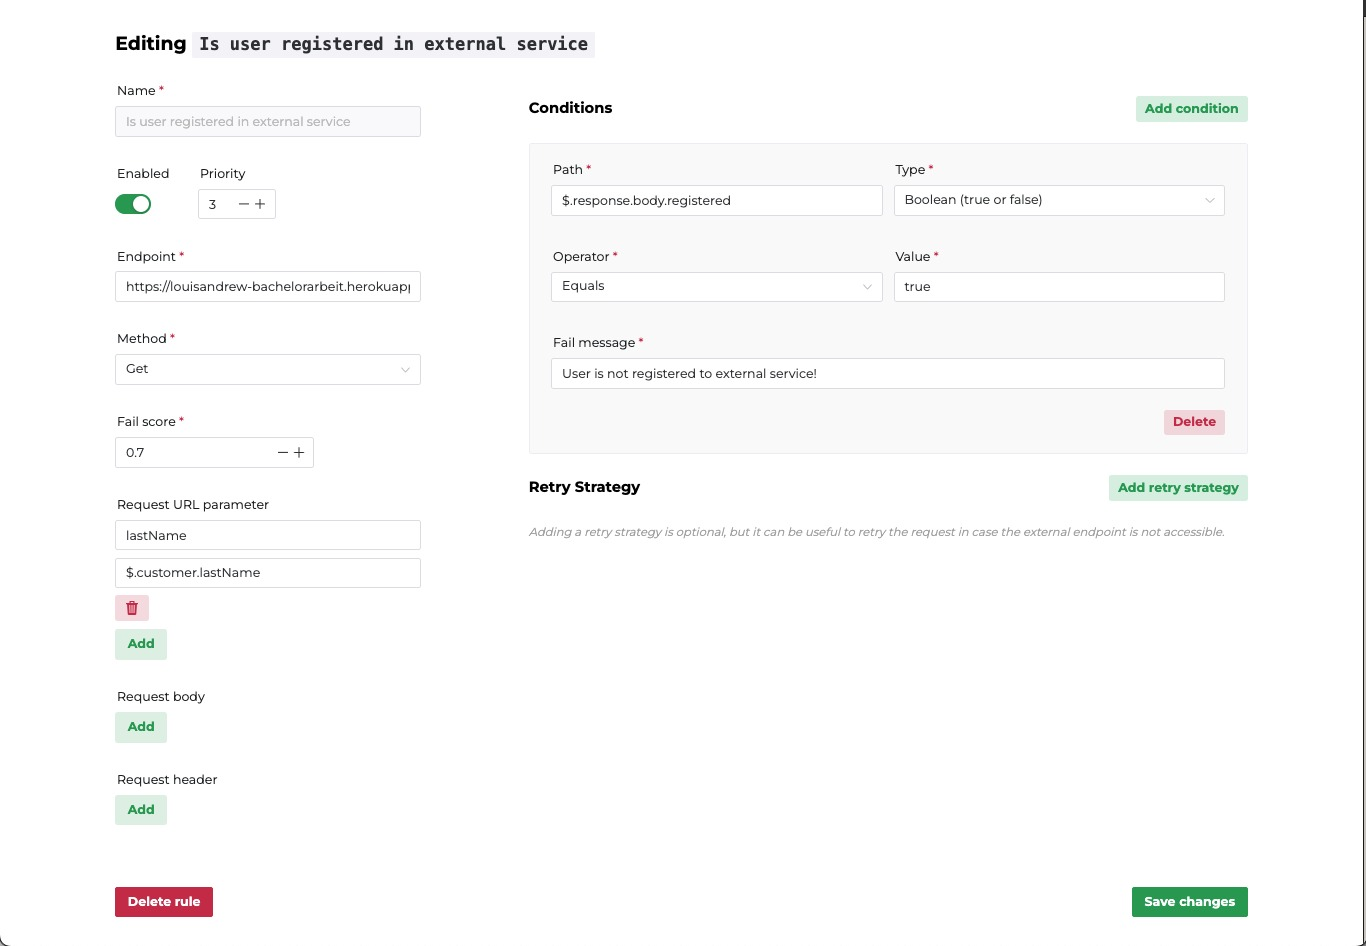
\includegraphics[width=\textwidth]{images/ss_sample_filled.jpeg}
      \caption{Screenshot of the rule management form}
    \end{figure}

    \subsubsection{Conditions Section}

      The \textsc{Conditions} section is a component, used to add one more condition to a validation rule. The \textsc{Conditions} section renders the list of conditions provided in a card, containing form fields for each attribute of the particular condition. Each card represents a single form, which also contains validation on its fields. 
      
      As mentioned before, the available values for the \verb;operator; attribute of a condition depends on its \verb;type; attribute. To prevent an invalid condition being sent to the FDS, the \textsc{Operator} field is a select field, and its options are defined by the current value inputted on the \textsc{Type} field. The intention of the restriction is to make sure that the \verb;operator; chosen is always valid to the corresponding \verb;type; of the condition.

      \begin{lstlisting}[style=es6, caption={Function to get list of available operators based on a condition's type attribute (TypeScript)}]
const getAvailableOperators = (type: ConditionType) => {
  switch (type) {
    case "string":
      return [
        { label: "Equals", value: "eq" },
        { label: "Starts with", value: "starts" },
        { label: "Includes", value: "incl" },
        { label: "Ends with", value: "ends" },
      ]
    case "number":
      return [
        { label: "Greater than", value: "gt" },
        { label: "Greater than equals", value: "gte" },
        { label: "Lesser than", value: "lt" },
        { label: "Leser than equals", value: "lte" },
        { label: "Equals", value: "eq" },
      ]
    case "array":
      return [
        { label: "Includes", value: "incl" },
        { label: "Excludes", value: "excl" },
        { label: "Number of items equals", value: "len" },
        { label: "Is empty", value: "empty" },
      ]
    case "boolean":
      return [{ label: "Equals", value: "eq" }]
    default:
      return []
  }
}
      \end{lstlisting}

      \begin{figure}[!ht]
        \centering
        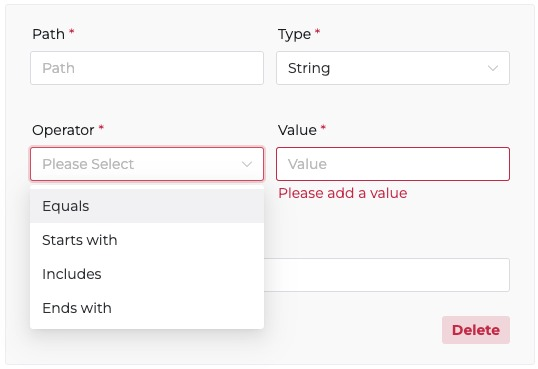
\includegraphics[width=0.8\textwidth]{images/ss_condition_op.jpeg}
        \caption{Screenshot of the "Operator" select field options, based on the current "Type" value}
      \end{figure}
      
      If more than one condition is provided, a radio field is also rendered, so that the user can choose one of the provided modifier for the list of conditions (either \textbf{\emph{ALL}} or \textbf{\emph{ANY}}). 

      A form validation is also implemented in the \textsc{Conditions} section. The validation not only make sure that all the required fields are filled, but also the value of the fields itself. For example, the validation will display an error message if the \textsc{Type} field is set to "Number", but the input value of the \textsc{Value} field is not a valid number. 

    \subsubsection{Autocomplete Input}

    A JSONPath expression is a valid value for some attributes of a \verb;ValidationRule;, and it also might be needed to access the current runtime information during a validation process, such as the HTTP response from the external endpoint, runtime secrets and customer information. Unfortunately, it might be difficult to memorize the expressions needed to access certain values, and it might also confuse the user. 

    \begin{figure}[!ht]
      \centering
      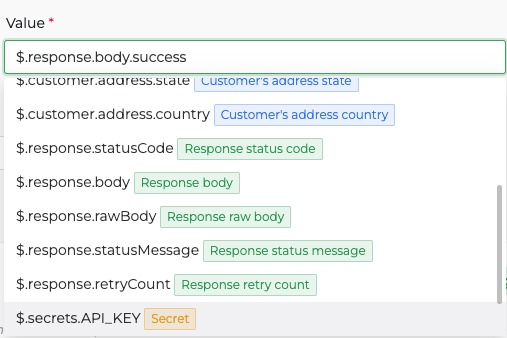
\includegraphics[width=0.5\textwidth]{images/ss_autocomplete.jpeg}
      \caption{Screenshot of the autocomplete input usage}
    \end{figure}

    To solve this problem, an autocomplete input field is provided in certain fields where a JSONPath expression is used. User can then display a list of possible JSONPath expressions by prefixing an input field with "\$", and choosing one of the expressions listed. User can also extend the expression chosen. The autocomplete input is used in the following form fields:

    \begin{itemize}
      \item \textsc{Path} field on \textsc{Conditions} section
      \item \textsc{Value} field on \textsc{Conditions} section
      \item Value field of a dynamic input\footnote{Autocompletion on \emph{\$.response} is not available here.}
    \end{itemize}

  \subsection{Validation Form}

    The validation form is a simple form similar to a customer registration form, specifically to mimic a new customer registration and to run a validation process directly after a new registration. Form validation is also implemented in the validation form to make sure that the customer information sent to the FDS is complete. A set of sample customers with specific characteristic is created to provide the functionality of pre-filling the validation form. 

    \begin{figure}[!ht]
      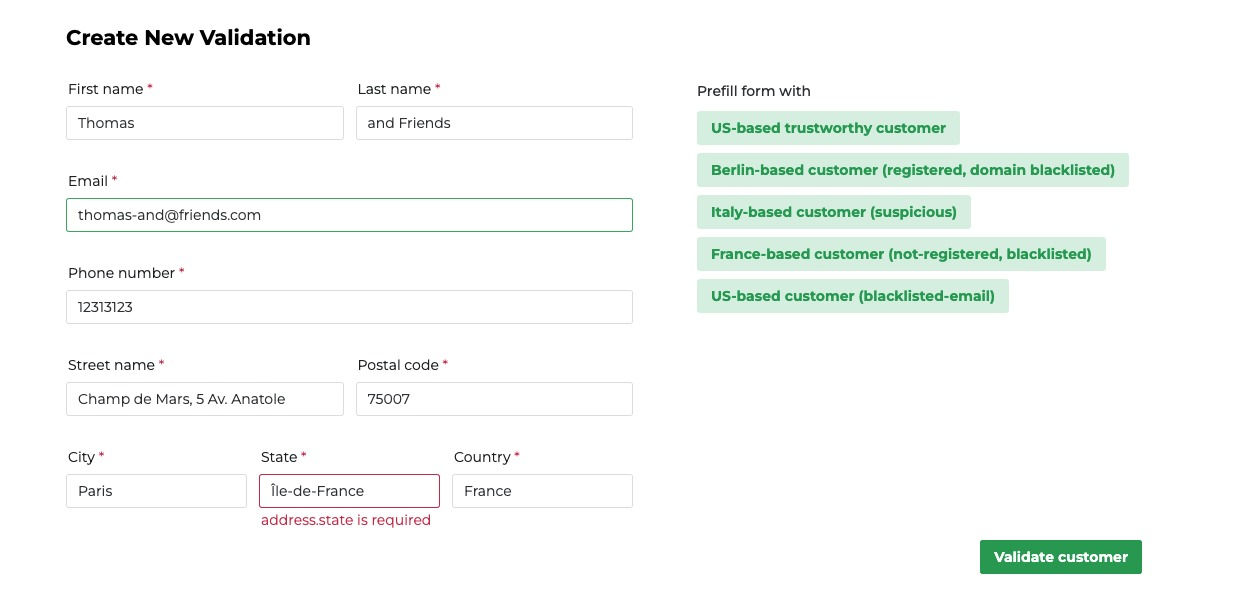
\includegraphics[width=\textwidth]{images/ss_customer_form.jpeg}
      \caption{Screenshot of the validation form}
    \end{figure}

    \begin{lstlisting}[style=es6, caption={Prefilling form values with a sample customer data (TypeScript)}]
const applySampleCustomer = (sampleCustomer: Customer) => {
  Object.assign(formValues, {
    ...sampleCustomer,
  })
}
    \end{lstlisting}

    When the user filled the fields properly and clicked the \textsc{Validate customer} button, the UI sends an HTTP POST request to the FDS with the customer data as the payload to schedule a new validation process. As the FDS returns an ID of the validation process, the UI will then redirect the user to the validation progress page, showing the validation progress in real time. 

    \begin{lstlisting}[style=es6, caption={ (TypeScript)}]
const { data } = await createNewValidation(customer)
if (data.validationId) {
  router.push(`/validations/${data.validationId}`)
}
    \end{lstlisting}

  \subsection{Validation Progress}
  
    To receive the real time event stream sent by the FDS as described in \autoref{impl_sse}, the \verb;EventSource; API can be used on the client side. With the \verb;EventSource; API, a persistent connection to the FDS will be opened, and the messages sent will be received by the client in real time. Because the FDS sends the messages as a string in an event stream, the UI has to parse the message content into a valid JSON object before processing it. 

    \begin{lstlisting}[style=es6, caption={Using the EventSource API in the browser (TypeScript)}]
const source = new EventSource(url)

source.onmessage = messageEvent => {
  try {
    const data = JSON.parse(messageEvent.data)
    // Do data processing
  } catch {
    // Handle error, if the message data is not a valid JSON object
  }
}
    \end{lstlisting}

    It is also important to close the connection to the event stream when it's no longer needed. The logic of closing the open connection when user leaves the current page is also implemented on the UI. 

    As the content of the message is parsed and identified as a valid \verb;ValidationResult; object, it is saved into the current state of the \verb;Validation; component, which renders the events of a validation process into a timeline component to give the user a better graphical overview of the current process. Vue3 uses the \emph{Proxy}\autocite[pp. 207-217]{gamma-1995} design pattern under the hood to provide a reactivity system on the UI, providing the possibility to update the timeline component every time a new validation result is published by the FDS. 

    \begin{figure}[!ht]
      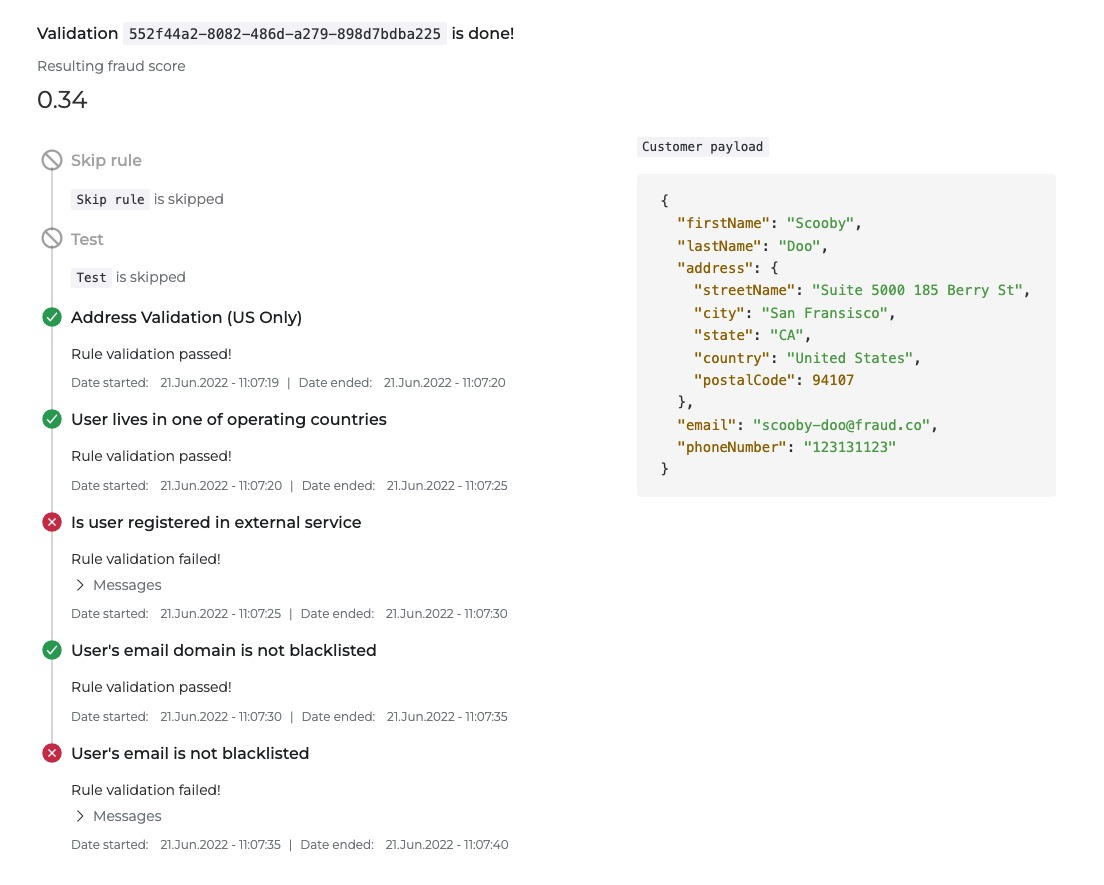
\includegraphics[width=\textwidth]{images/ss_validation_progress.jpeg}
      \caption{Screenshot of the validation progress in real time}
    \end{figure}

    The ID of the validation as well as the current fraud score of a validation process are always displayed, to give detailed information to the user regarding the current validation process. Additionally, the customer data is also displayed as a JSON object, to give the user with technical knowledge a better overview on the data being sent to the FDS. 
  
  \subsection{Runtime Secrets}

    A component to display a list of the available runtime secrets in a dialog is also created. For security purposes, only the key of the secrets are displayed within the component. The component also provides a possibility to create a new runtime secret and to delete an existing secret. User can create a new secret by clicking on the \textsc{Create a new secret} button, and adding the essential information on the form fields displayed. To delete an existing secret, a \textsc{Delete} button is displayed next to each secret's key name. The list of available runtime secret keys are also accessible on the autocomplete options, making it easier for the user to access the appropriate secret key without having to memorize the key name.
    
    \begin{figure}[!ht]
      \centering
      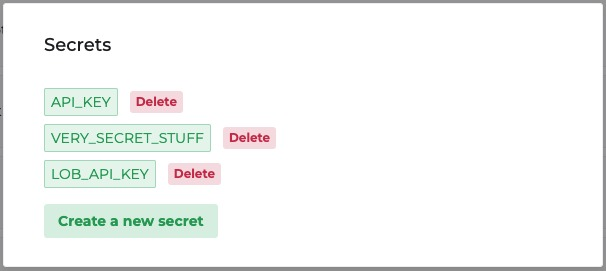
\includegraphics[width=0.6\textwidth]{images/ss_secrets.jpeg}
      \caption{Screenshot of a component to list available runtime secrets}
    \end{figure}
    

Optionals:
\begin{itemize}
  \item Architecture -> (can be in controller)
  \item Techs 
\end{itemize}
\chapter{Test}

  Testing is an integral part of software development. Writing tests gives the developer the confidence that the recent changes made will not break the remaining parts of the software. The system is built by writing the tests before implementing the particular features (also known as \emph{TDD} method), in hope that the tests can help reduce the amount of bugs in the system while also providing a code-level working specification of the particular component. The technology used to run test suites for both the FDS and the UI is \emph{vitest}\footnote{\emph{Vitest} is a unit test framework, with out-of-box TypeScript support and Vite native compatibility. GitHub repository: \url{https://github.com/vitest-dev/vitest}.}. This chapter discusses the tests written during the development process.

  \section{Unit Test}


  \begin{itemize}
   \item FDS -> unit test to make sure that all components are working correctly
   \item FDS example condition evaluator
   \item UI -> Testing the behavior of the UI rather than functionality
   \item UI -> Testing simple components, example is key-value input
  \end{itemize}

  \section{Integration Test}

  \begin{itemize}
   \item Integration on FDS -> Endpoint test
   \item Use superagent and on
   \item UI -> Check that usage of other components are ok, minimal mocking
  \end{itemize}
\chapter{Darstellung und Bewertung der Ergebnisse}
[Beschreibung der Ergebnisse aus allen voran gegangenen Kapiteln sowie der zuvor generierten Ergebnisartefakte mit Bewertung, wie diese einzuordnen sind]


\section{Ausblick}
[Beschreibung und Begr\"undung potenzieller zuk\"unftiger Folgeaktivit\"aten im Zusammenhang mit Ihrer Arbeit (z.B. weitere Anforderungen, Theoriebildung, ... ]



\printbibliography[
  heading=bibintoc,
  title={Bibliography}
]

\newpage

\chapter{List of Abbreviations}
\newpage

\chapter{Glossary}

\appendix
\pagenumbering{Roman}

\chapter{Appendix}


 \section{Supplemental Figures}

  \begin{figure}[!ht]
   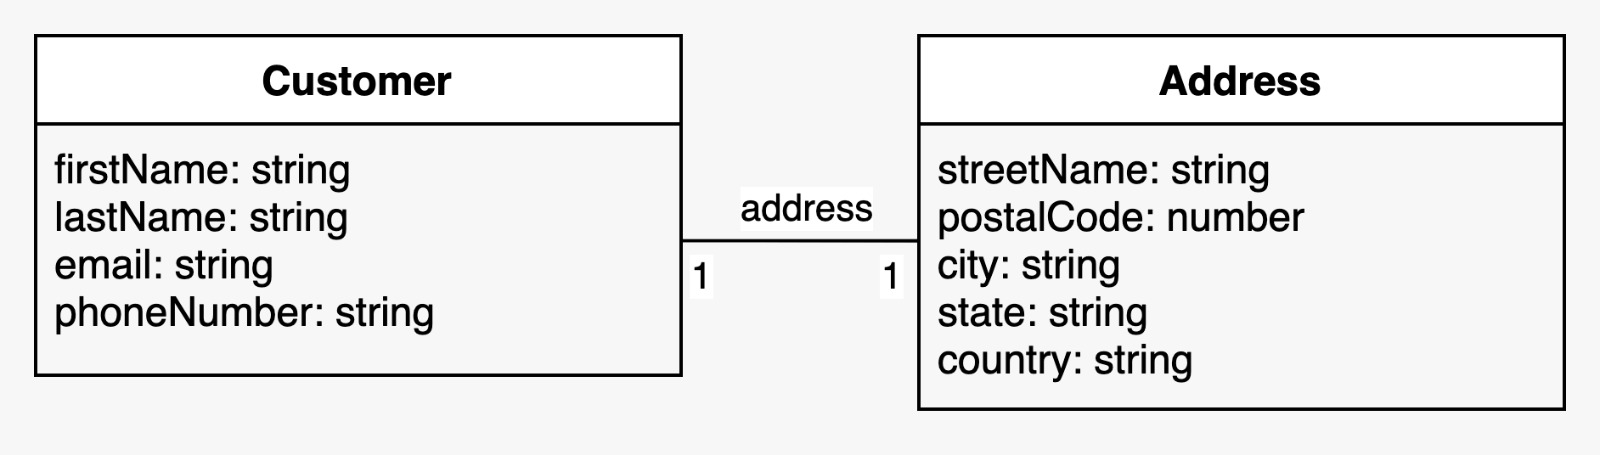
\includegraphics[width=\textwidth]{diagrams/entity_customer.jpeg}
   \caption{UML diagram of the customer model}
   \label{fig:customer_uml}
  \end{figure}

 \section{Supplemental Source Codes}
 
  \begin{lstlisting}[caption={\emph{Prisma} schema of a validation rule (Prisma)}, label={code:prisma}]
 model ValidationRule {
   id                  String    @id @default(auto()) @map("_id") @db.ObjectId
   name                String    @unique
   skip                Boolean
   priority            Int
   endpoint            String
   method              String
   failScore           Float
   condition           Json
   retryStrategy       Json?
   requestUrlParameter Json?
   requestBody         Json?
   requestHeader       Json?
 }
  \end{lstlisting}

\section{Quell-Code}

\section{Tipps zum Schreiben Ihrer Abschlussarbeit}

\begin{itemize}
\item Achten Sie auf eine neutrale, fachliche Sprache. Keine \glqq{}Ich\grqq{}-Form.
\item Zitieren Sie zitierf\"ahige und -w\"urdige Quellen (z.B. wissenschaftliche Artikel und Fachb\"ucher; nach M\"oglichkeit keine Blogs und keinesfalls Wikipedia\footnote{Wikipedia selbst empfiehlt, von der Zitation von Wikipedia-Inhalten im akademischen Umfeld Abstand zu nehmen \autocite{wikipedia2019}.}). 
\item Zitieren Sie korrekt und homogen.
\item Verwenden Sie keine Fu{\ss}noten f\"ur die Literaturangaben.
\item Recherchieren Sie ausf\"uhrlich den Stand der Wissenschaft und Technik.
\item Achten Sie auf die Qualit\"at der Ausarbeitung (z.B. auf Rechtschreibung).
\item Informieren Sie sich ggf. vorab dar\"uber, wie man wissenschaftlich arbeitet bzw. schreibt:
\begin{itemize}
\item Mittels Fachliteratur\footnote{Z.B. \autocite{balzert2011}, \autocite{franck2013}}, oder
\item Beim Lernzentrum\footnote{Weitere Informationen zum Schreibcoaching finden sich hier: \url{https://www.htw-berlin.de/studium/lernzentrum/studierende/schreibcoaching/}; letzter Zugriff: 13 VI 19.}.
\end{itemize}
\item Nutzen Sie \LaTeX\footnote{Kein Support bei Installation, Nutzung und Anpassung allf\"alliger \LaTeX-Templates!}.
\end{itemize}



\newpage
% Letzte Seite
\thispagestyle{empty}      
\noindent

\newpage
\section*{Eidesstattliche Versicherung}
Hiermit versichere ich an Eides statt durch meine Unterschrift, dass ich die vorstehende Arbeit selbstst\"andig und ohne fremde Hilfe angefertigt und alle Stellen, die ich w\"ortlich oder ann\"ahernd w\"ortlich aus Ver\"offentlichungen entnommen habe, als solche kenntlich gemacht habe, mich auch keiner anderen als der angegebenen Literatur oder sonstiger Hilfsmittel bedient habe. Die Arbeit hat in dieser oder \"ahnlicher Form noch keiner anderen Pr\"ufungsbeh\"orde vorgelegen.\\
\linebreak[4]
\linebreak[4]
\linebreak[4]
\linebreak[4]
-------------------------------------------------------\linebreak[4]
22.07.2022, Berlin



\end{document}

